\documentclass[11pt]{article}
\usepackage{csquotes}
\usepackage{graphicx}
\usepackage{hyperref}
\usepackage[utf8]{inputenc}
\usepackage{amsmath,amsthm,amsfonts,amssymb,amscd}
\usepackage{tikz}
\usepackage{xeCJK}
\usepackage{physics}
\usepackage{multirow,booktabs}
% \usepackage[table]{xcolor}
\usepackage{fullpage}
\usepackage{lastpage}
\usepackage{unicode-math}
\usepackage{enumitem}
\usepackage{fancyhdr}
\usepackage{mathrsfs}
\usepackage{wrapfig}
\usepackage{setspace}
\usepackage{calc}
\usepackage{multicol}
\usepackage{cancel}
\usepackage[retainorgcmds]{IEEEtrantools}
\usepackage[margin=3cm]{geometry}
\usepackage{amsmath}
\DeclareMathAlphabet{\mathcal}{OMS}{cmsy}{m}{n}
\let\mathbb\relax
\DeclareMathAlphabet{\mathbb}{U}{msb}{m}{n}
\newlength{\tabcont}
\setlength{\parindent}{0.0in}
\setlength{\parskip}{0.05in}
\usepackage{empheq}
\usepackage{framed}
\usepackage[most]{tcolorbox}
\usepackage{xcolor}
\linespread{1.2}
\graphicspath{{./}}
\setCJKmainfont[AutoFakeBold = 3, AutoFakeSlant = 4]{BiauKaiTC}
\colorlet{shadecolor}{orange!15}
\parindent 0in
\parskip 12pt
\geometry{margin=1in, headsep=0.25in}
\theoremstyle{definition}
\newtheorem{thr}{Theorem}
\newtheorem{defn}{Definition}
\newtheorem{reg}{Rule}
\newtheorem{exer}{Exercise}
\newtheorem{note}{Note}
\newtheorem{asmp}{Assumption}
\begin{document}
\setcounter{section}{0}
\title{Title}

\thispagestyle{empty}
\begin{center}
  {\large \bf HTML HW1} \\ 
  B12901022 廖冠豪
\end{center}
\section*{5}
The answer by the agent is as follows
% \begin{itemize}
%   \item medical image classification 
%   \item Natural language processing tasks (e.g., text classification, sentiment analysis)
%   \item Autonomous driving (e.g., labeling road scenes with uncertain or rare conditions)
%   \item Fraud detection in financial systems
% \end{itemize}
\begin{displayquote}
% A possible application of active learning is in medical image analysis. In this context, labeling medical images (like MRI scans or X-rays) requires expert knowledge, often provided by radiologists, making the labeling process expensive and time-consuming. Active learning can help by selecting the most informative images for labeling, reducing the number of images that need to be manually labeled while still improving the performance of a machine learning model.
% This approach optimizes the use of expert resources and accelerates model training, making it particularly useful for early-stage AI-assisted diagnostic systems.
  Active learning is a machine learning approach where the model is trained interactively by selecting the most informative data points from which to learn, rather than being trained on a large set of randomly selected data. This can be particularly useful when labeled data is scarce or expensive to obtain.

One possible application of active learning is in medical image classification. Medical experts' time is expensive, and annotating images like X-rays, MRIs, or CT scans can be labor-intensive. In an active learning scenario, a machine learning model would initially be trained on a small labeled dataset. As the model identifies new cases where it is uncertain, it queries the experts to label these specific cases. Over time, the model improves its performance while minimizing the number of images that need manual labeling, leading to cost and time efficiency. \\ 
Other applications of active learning include:
  \begin{itemize}
    \item Natural language processing tasks (e.g., text classification, sentiment analysis)
    \item Autonomous driving (e.g., labeling road scenes with uncertain or rare conditions)
    \item Fraud detection in financial systems
  \end{itemize}
\end{displayquote}
I agree mostly with the agent's answer. Active learning is suitable for cases in which unlabeled is abundant but manual labeling is expensive. All the answers provided by the agent fits this criteria. Unlabeled data is abundant in these cases, but labeling requires human expertise, which can be costly. The agent further explains how active learning can be used to tackle these cases. The active learning model asks the human expert when encountering a data case of which it is unsure. It's performance improves during the process and the number of queries to human experts is minimized. The one thing I don't like about the agent's answer is that it doesn't provide any real-life examples in which active learning is actually applied to any of the cases it mentioned. This is a flaw to me because when being asked what "applications" active learning has the expected answer should fields in which active learning is actually used and contributing, instead of cases that theoretically would be a suitable problem for active learning. In conclusion, as the agent's boss, I'm mostly satisfied with the answer it provides, but this satisfaction is compensated by the lack of real-life example in it's answer.
\newpage
\section*{6}
The answer by the agent is as follows(some content that isn't directly related to the question is omitted)
\begin{displayquote}
  While machine learning (ML) has potential in predicting aspects of earthquake activity, it is still not fully reliable for precise earthquake predictions. The unpredictable nature of seismic events, combined with the complexity of underlying geological processes, makes earthquake prediction a highly challenging task. \\ 
  Challenges
  \begin{itemize}
    \item Lack of sufficient labeled data: While seismic data is abundant, labeled data for events directly leading to earthquakes is rare and often ambiguous.
    \item Complexity of Earth systems: The geological processes underlying earthquakes are extremely complex and not fully understood, limiting the ability of even the most advanced models.
  \end{itemize}
\end{displayquote}
I agree with the agent's answer. The difficulties in trying to precisely predict earthquake events is clearly marked in the answer. First, it's hard to obtain well-labeled data for the model to train from, as the causes of earthquakes is still not fully known to human experts. Therefore, the reliability of the data cannot be guaranteed. As we've learned from the lecture, the No Free Lunch Theorem states that no meaningful result can be produced by learning without correct assumption. Given that scientists have not a complete understanding of the mechanism behind earthquakes, it's hard to make the "correct assumption". Second, given the complex geological nature, all earthquakes might not share a common cause. It might be that multiple different geological phenomenons can all lead to earthquakes. If this is the case, it would be hard to train a model to predict earthquakes by recognizing underlying common patterns, as there could be none. In conclusion, as the agent's boss, I agree with and am satisfied with the answer provided, as the argument is clear and fits my understanding of geology.
\newpage
\section*{7}
In this problem, we set sign(0) = 1. \\ 
Consider the case where
\begin{gather*}
  N = 1, 
  \vb{x}_1^\text{orig} =
  \begin{bmatrix}
    1 \\ 
    1 
  \end{bmatrix}, 
  y_1 = -1
\end{gather*}
We first run PLA on ${(\vb{x}_n, y_n)}_{n = 1}^1$. Since $\text{sign}(\vb{w}_0^T\vb{x}_1) = 1 \neq y_1$, $\vb{w}$ is updated by
\begin{gather*}
  \vb{w}_1\leftarrow\vb{w}_0 + y_1\vb{x}_1 \\ 
  \implies \vb{w}_1 = \begin{bmatrix}
    -2 \\
    -1 \\ 
    -1
  \end{bmatrix}
\end{gather*}
After this update, there are no more mistakes, so the algorithm returns
\[
  \vb{w}_\text{PLA} = \begin{bmatrix}
    -2 \\ 
    -1 \\
    -1
  \end{bmatrix}
\]
We then run PLA on ${(\vb{x}^\prime_n, y_n)}_{n = 1}^1$. Since $\text{sign}(\vb{w}_0^T\vb{x}^\prime_1) = 1 \neq y_1$, $\vb{w}$ is updated by
\begin{gather*}
  \vb{w}_1\leftarrow\vb{w}_0 + y_1\vb{x}^\prime_1 \\ 
  \implies \vb{w}_1 = \begin{bmatrix}
    -1 \\
    -1 \\ 
    -1
  \end{bmatrix}
\end{gather*}
After this update, there are no more mistakes, so the algorithm returns
\[
  \vb{w}^\prime_\text{PLA} = \begin{bmatrix}
    -1 \\ 
    -1 \\
    -1
  \end{bmatrix}
\]
We then consider the example in $\mathbb{R}^2$
\[
  \vb{x}_\text{ex}^\text{orig} = \begin{bmatrix}
    -1 \\ 
    0 \\
  \end{bmatrix}
\]
We see that 
\begin{gather*}
  \text{sign}(\vb{w}_\text{PLA}^T\vb{x}_\text{ex}) = \text{sign}(-1 + 1 + 0) = 1 \\ 
  \text{sign}(\vb{w}_\text{PLA}^{\prime T}\vb{x}_\text{ex}) = \text{sign}(-2 + 1 + 0) = -1 \\
\end{gather*}
Hence $\vb{w}_\text{PLA}$ and $\vb{w}_\text{PLA}^\prime$ don't always return the same binary classification for examples $\vb{x}^\text{orig} \in \mathbb{R}^2$, and the statement is disproved.
\newpage
\section*{8}
In this problem, we set sign(0) = 1. \\ 
We first prove that \textbf{mistakes happen at the same values of $t$ for the two processes} by mathematical induction. Let $\vb{w}_t^\prime$ and $\vb{w}_t$ the weight vector at the $t$-th step of the two processes running on ${(\vb{x}^\prime_n, y_n)}^N_{n=1}$ and ${(\vb{x}_n, y_n)}^N_{n=1}$ respectively. \\
At $t = 0$ $\vb{w}^\prime_0 = \vb{w}_0 = \vb{0}$. \\ 
Suppose that from $t=0$ to $t=t^\prime$ all the mistakes (and updates) happen at $t\in\mathcal{T} = \{t_1, t_2,... t_k\}$ for the two processes. \\ 
Hence we have
\begin{gather*}
  \vb{w}^\prime_{t^\prime} = \sum_{t\in\mathcal{T}}y_t(3, 3\vb{x}_t^\text{orig}) \\ 
  \vb{w}_{t^\prime} = \sum_{t\in\mathcal{T}}y_t(1, \vb{x}_t^\text{orig}) \\ 
  \implies \vb{w}^\prime_{t^\prime} = 3\vb{w}_{t^\prime}
\end{gather*}
And
\[
  \text{sign}(\vb{w}^{\prime T}_{t^\prime}\vb{x}) = \text{sign}(\vb{w}_{t^\prime}^T\vb{x}^\prime) \quad \forall \vb{x} = (1, \vb{x}^\text{orig}), \vb{x}^\prime = (3, 3\vb{x}^\text{orig}), \vb{x}^\text{orig}\in\mathbb{R}^d
\]
Therefore, the next test ($t = t^\prime + 1$) is a mistake to either none or both of the processes, and the statement still holds. \\ 
By the analysis presented above, we now know that $\vb{w}_\text{PLA}^\prime = 3\vb{w}_\text{PLA}$, and they return the same binary classification result for any $\vb{x}^\text{orig} \in \mathbb{R}^d$, and are equivalent.
\newpage
\section*{9}
Define the $d + 1$-dimensional vector $\vb{w}_f$ based on the dictionary by 
\begin{gather*}
  {\vb{w}_f}_0 = -3.5 \\ 
  {\vb{w}_f}_i = \begin{cases}
    1 , & \text{if the $i$-th word in the dictionary is more hatred-like}\\
    -1 , & \text{if the $i$-th word in the dictionary is less hatred-like}
  \end{cases} \quad \text{for $1 \leq i \leq d$}
\end{gather*}
We have 
\[
  f(\vb{x}) = \text{sign}(\vb{w}_f^T\vb{x})
\]
So $\vb{w}_f$ is the perfect vector the PLA algorithm hopes to approximate. \\ 
We then consider the update process of $\vb{w}$ \\ 
First we consider the inner product of $\vb{w}_t$ and $\vb{w}_f$ 
\begin{gather*}
  \vb{w}_f^T\vb{w}_{t+1} = \vb{w}_f^T(\vb{w}_t + y_{n(t)}\vb{w}_t) \\ 
  \geq \vb{w}_f^T\vb{w}_t + \min_n(y_n\vb{w}_f^T\vb{x}_n)
\end{gather*}
Also, 
\begin{gather*}
  y_n\vb{w}_f^T\vb{x}_n = \left |f(\vb{x}_n)\right| \\
  \implies \min_n(y_n\vb{w}_f^T\vb{x}_n) = \min_n\left |z_+(\vb{x}_n) - z_-(\vb{x}_n) - 3.5\right| \geq \frac{1}{2} \quad(z_+(\vb{x}), z_-(\vb{x})\in\mathbb{N})
\end{gather*}
Therefore starting from $\vb{w}_0 = \vb{0}$, after $T$ updates(mistakes), we have
\[
  \vb{w}_f^T\vb{w}_T \geq \frac{T}{2}
\]
Next, we consider the change of the length of $\vb{w}_t$. 
\begin{gather*}
  \norm{\vb{w}_{t+1}}^2 = \norm{\vb{w}_t + y_{n(t)}\vb{x}_{n(t)}}^2 \\ 
  = \norm{\vb{w}_t}^2 + 2y_{n(t)}\vb{w}_t^T\vb{x}_{n(t)} + \norm{\vb{x}_{n(t)}}^2
  \leq \norm{\vb{w}_t}^2 + \max_n({\vb{x}_n}^2)
\end{gather*}
In this case we know that $\vb{x}$ has $m + 1$ components that equal to $1$ and others equal to $0$, so $\norm{x_n}^2 = m+1$
\begin{gather*}
  \implies \norm{\vb{w}_{t+1}}^2 \leq \norm{\vb{w}_t}^2 + (m + 1)
\end{gather*}
Therefore, starting from $\vb{w}_0 = \vb{0}$, after $T$ updates we have 
\[
  \norm{\vb{w}_T}^2 \leq T(m + 1)
\]
We finally consider the cosine of the angle between $\vb{w}_f$ and $\vb{w}$ after $T$ updates
\begin{gather*}
  \frac{\vb{w}_f^T\vb{w}}{\norm{\vb{w}_f}\norm{\vb{w}}} \geq \frac{T}{2\sqrt{T(m+1)}}\frac{1}{\norm{\vb{w}_f}} \\ 
  = \frac{1}{2\norm{\vb{w}_f}}\sqrt{\frac{T}{m+1}} \\
  = \sqrt{\frac{T}{4(m + 1)(d + 3.5^2)}}
\end{gather*}
We also know that the cosine value has to be no greater than $1$, so 
\begin{gather*}
  \sqrt{\frac{T}{4(m + 1)(d + 3.5^2)}} \leq 1 \\ 
  \implies T \leq (m + 1)^2(4d^2 + 49)
\end{gather*}
We hence obtain the upper bound for the number of mistakes this PLA algorithm can make.
\newpage
\section*{10}
% Histogram:
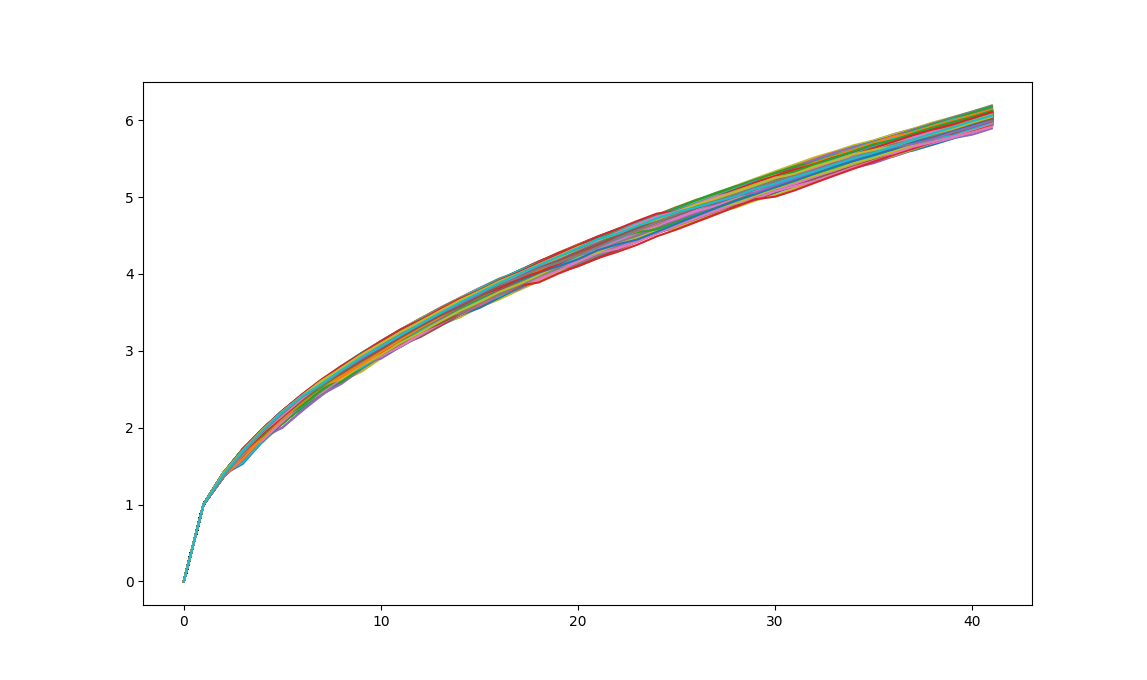
\includegraphics{P10_figure.png} \\
From the diagram presented above we see that throughout the $1000$ experiments, the number of updates mainly lies between $100$ and $105$. The number of experiments with a total update count outside of this interval decreases rapidly as it gets further away from this interval. Also, we see that the decrease on the side $n < 100$ is quite smooth, with the minimal total update count of the experiments being around $75$. On the other side, $n > 105$, the decrease is a lot more sharp, as the maximal total update count is no greater than $115$. We can also see that the distribution of the total number of updates approximates a right-shifted normal distribution. \\
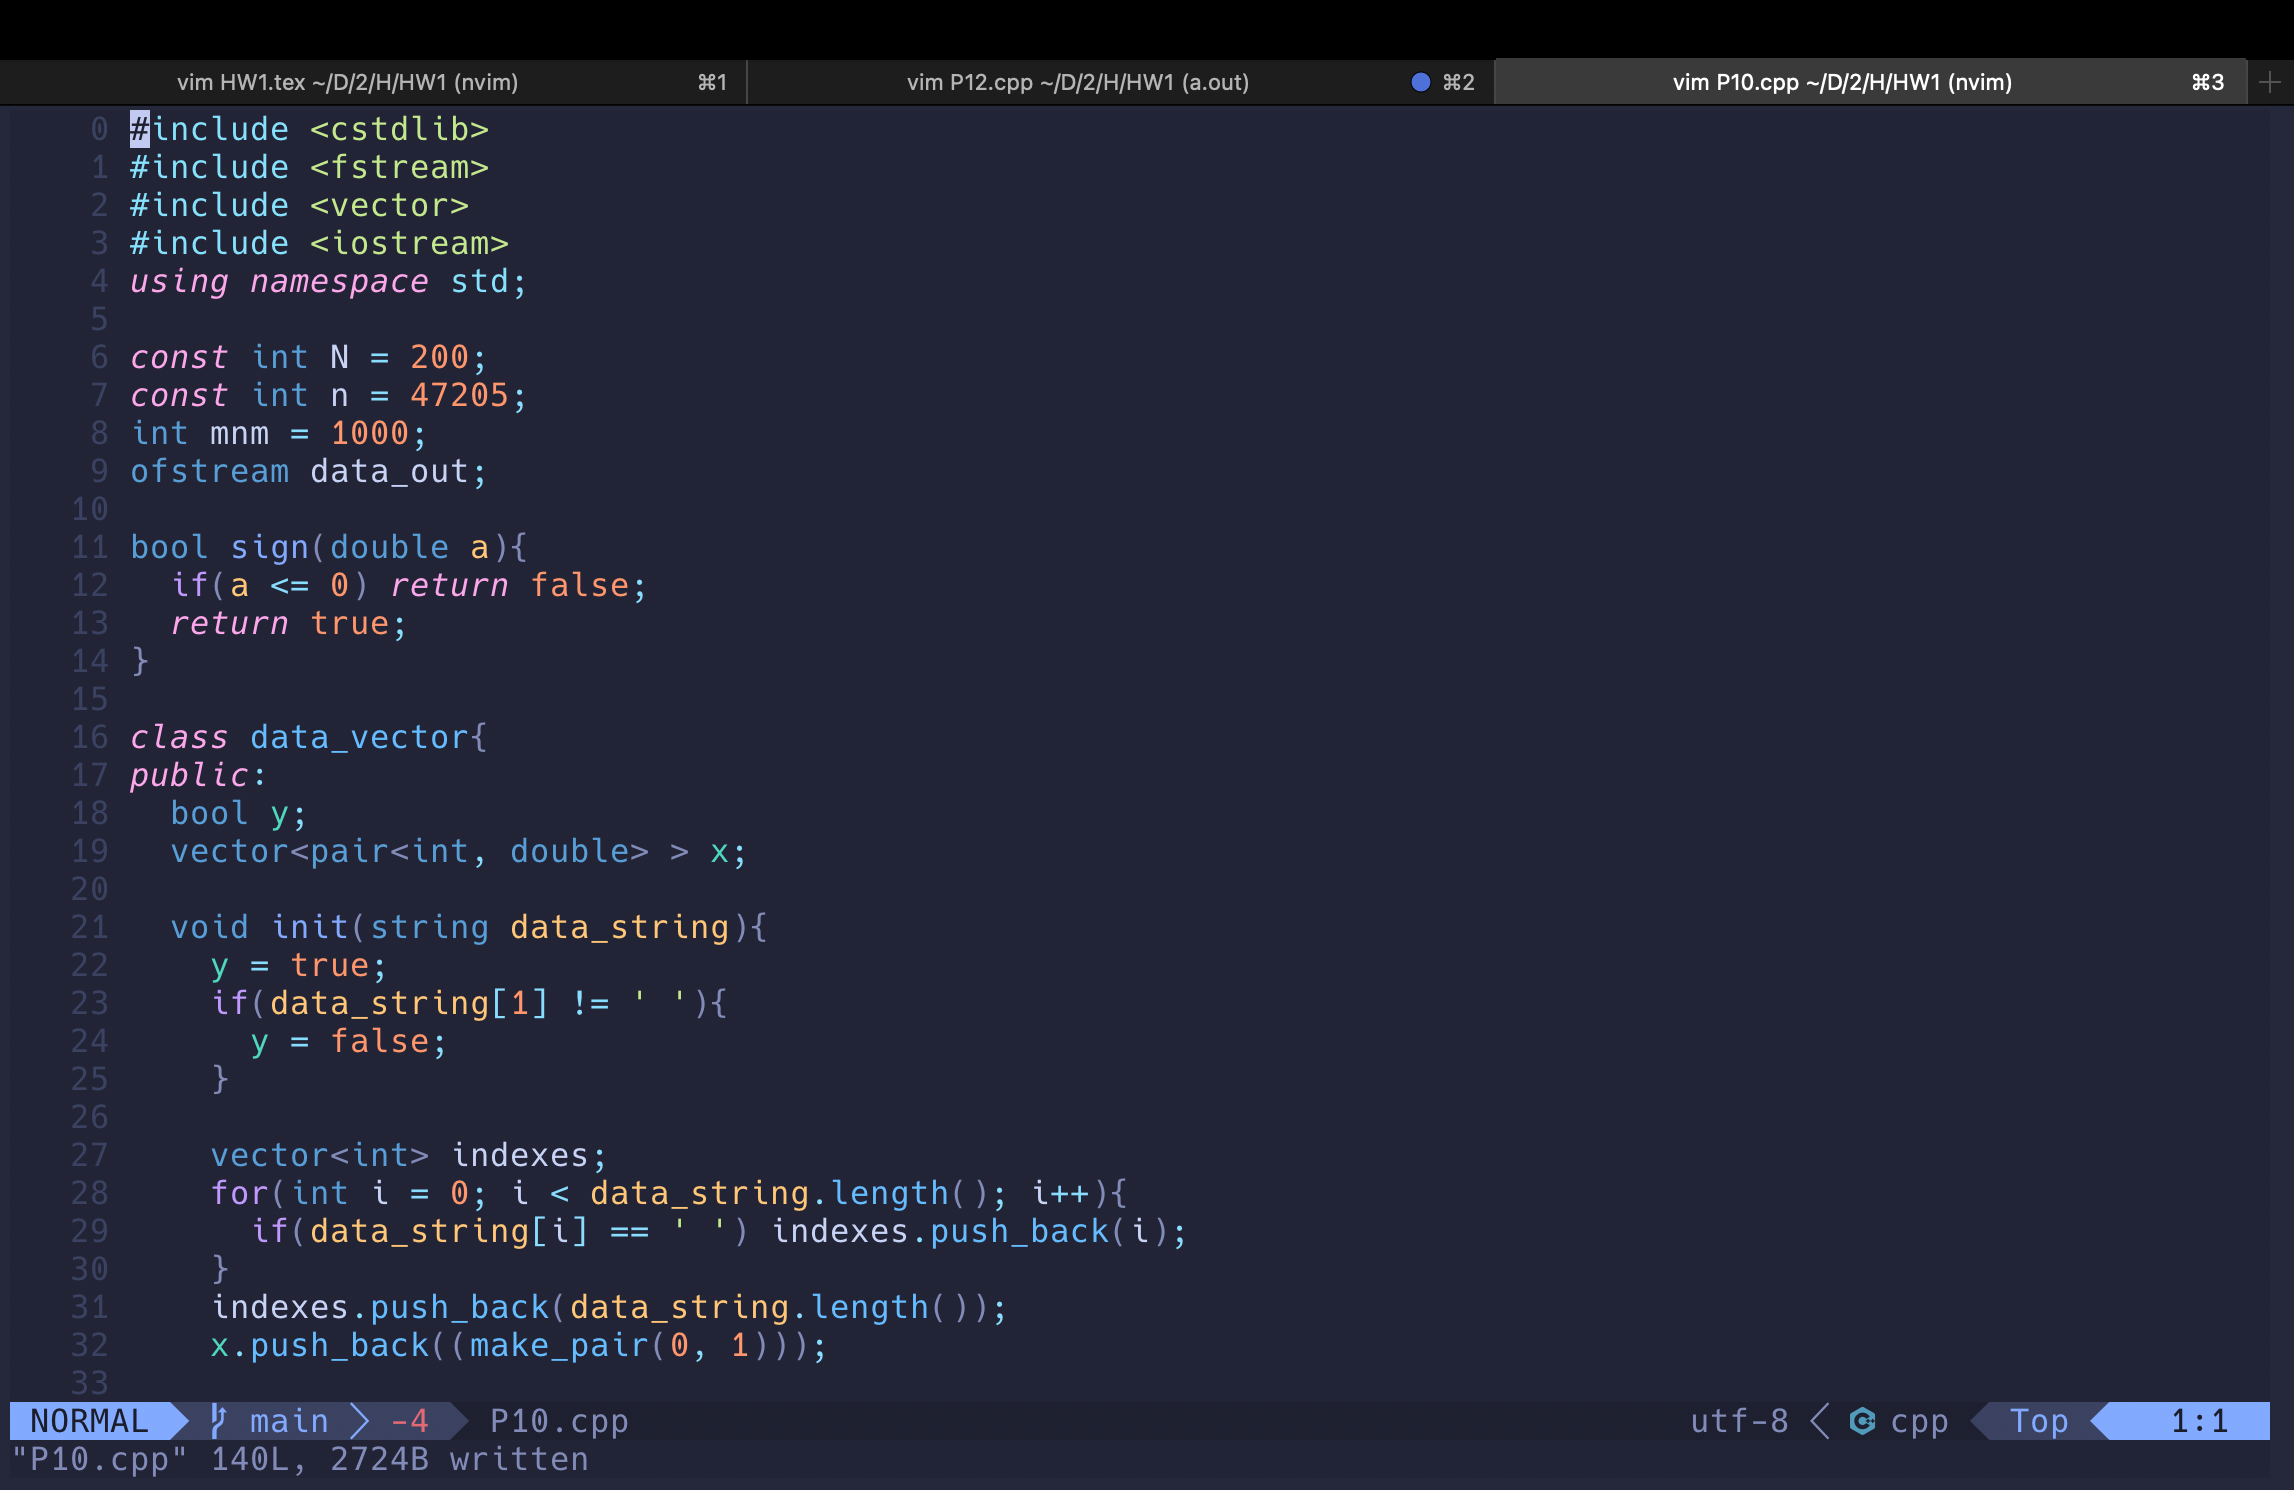
\includegraphics[width = \textwidth]{P10_code.png}\\
Code snapshot\\
\newpage
\section*{11}
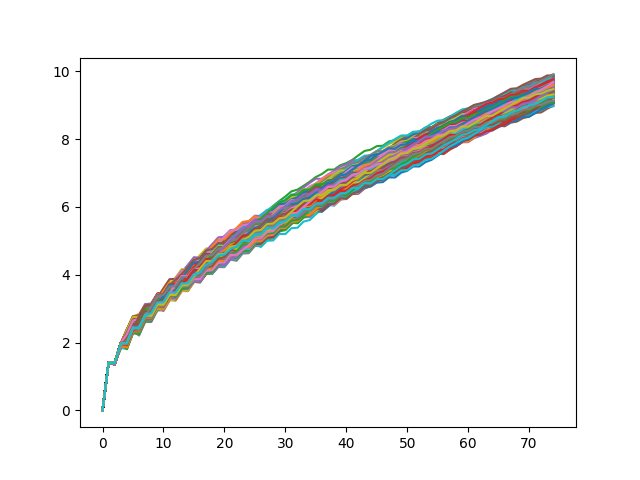
\includegraphics{P11_figure.png} \\
\textbf{$T_{min}$ = 74} \\
From the diagram presented above we see that the length of $\vb{w}$ is not always growing, with many small fluctuations during the process, but overall the  length is increasing, starting from $\norm{\vb{w}_0} = 0$ to $\norm{\vb{w}_{T_{min}}} \approx 10$. Also, the growth of $\vb{w}$ is a lot more rapid at the beginning of the process compared with the rest of the process. 
% A possible explanation is that since $\norm{\vb{w}}$ is small at the beginning, it's less likely that the effect of $y_{n(t)}\vb{x}_{n(t)}$ is compensated by a component of $\vb{w}_t$. \\
\newline
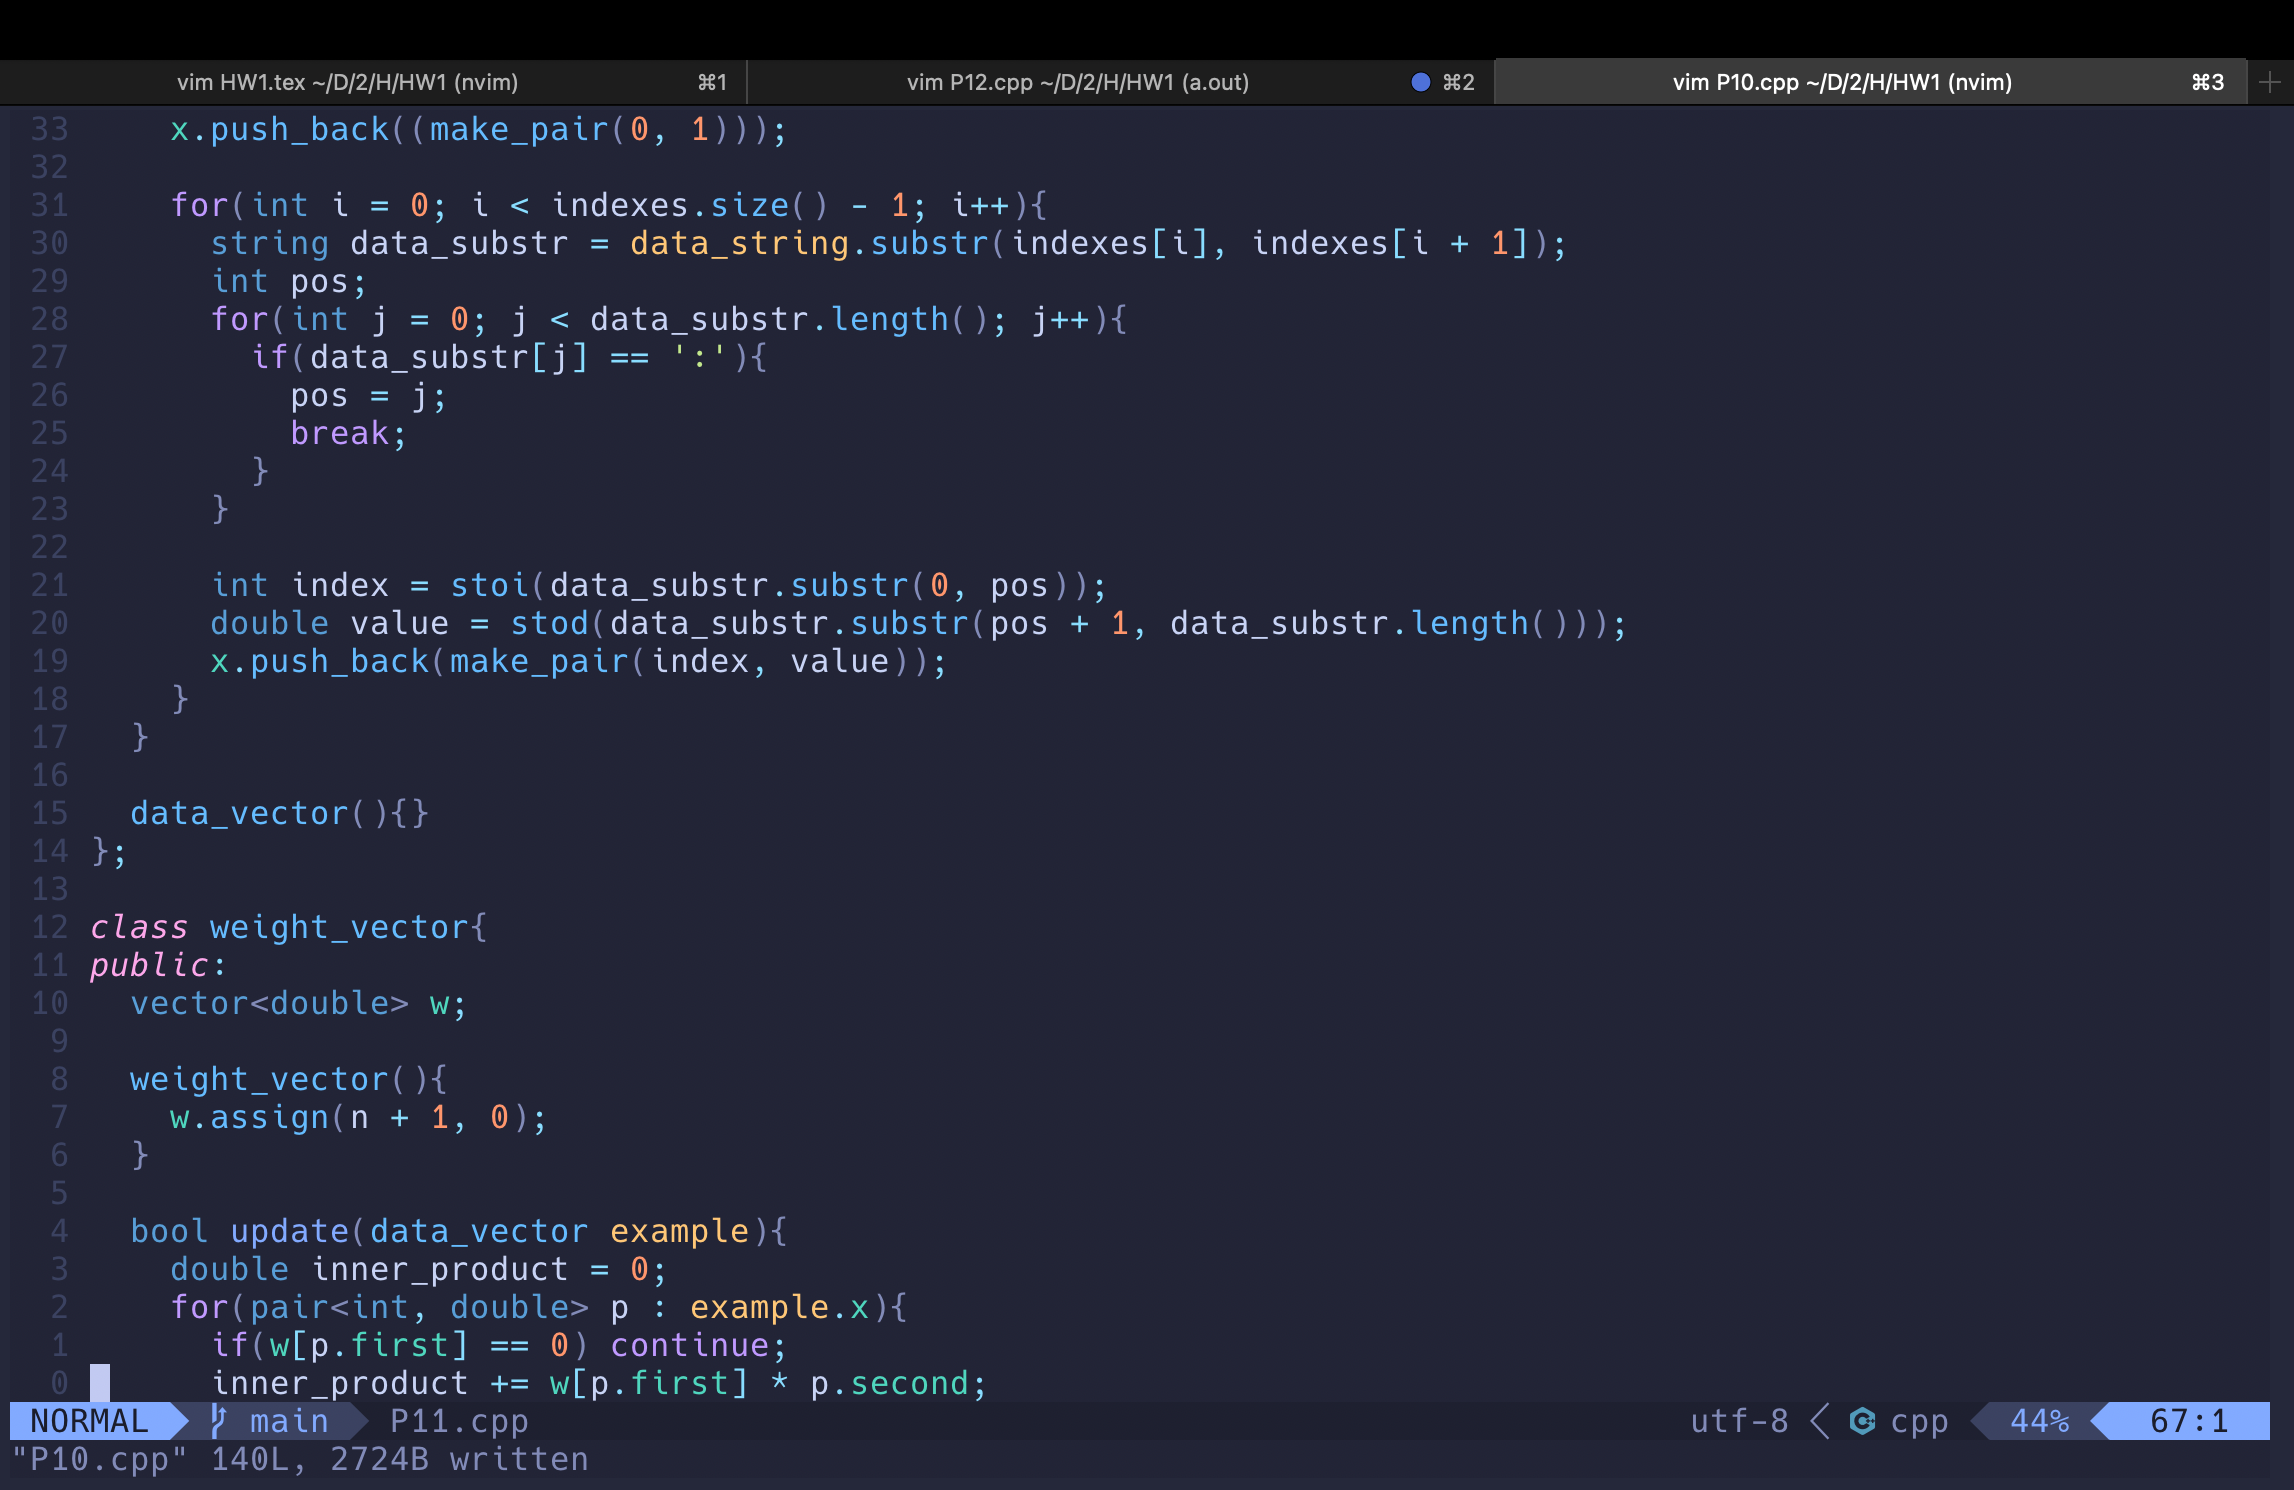
\includegraphics[width = \textwidth]{P11_code.png}\\
Code snapshot\\ 
\newpage
\section*{12}
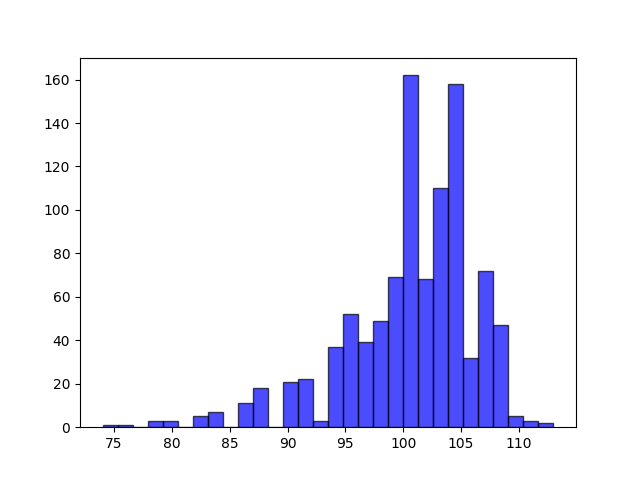
\includegraphics{P12_figure.png} \\
The median of number of updates is $101$. \\ 
Comparison between Problem 10: \\ 
We run the $1000$ experiments for $100$ times, in every process the two PLA variants use the same random seed, but the seed is different among all processes. We compare the two PLA variants by comparing the median of number of updates in the $100$ sets of experiments. \\
\newline
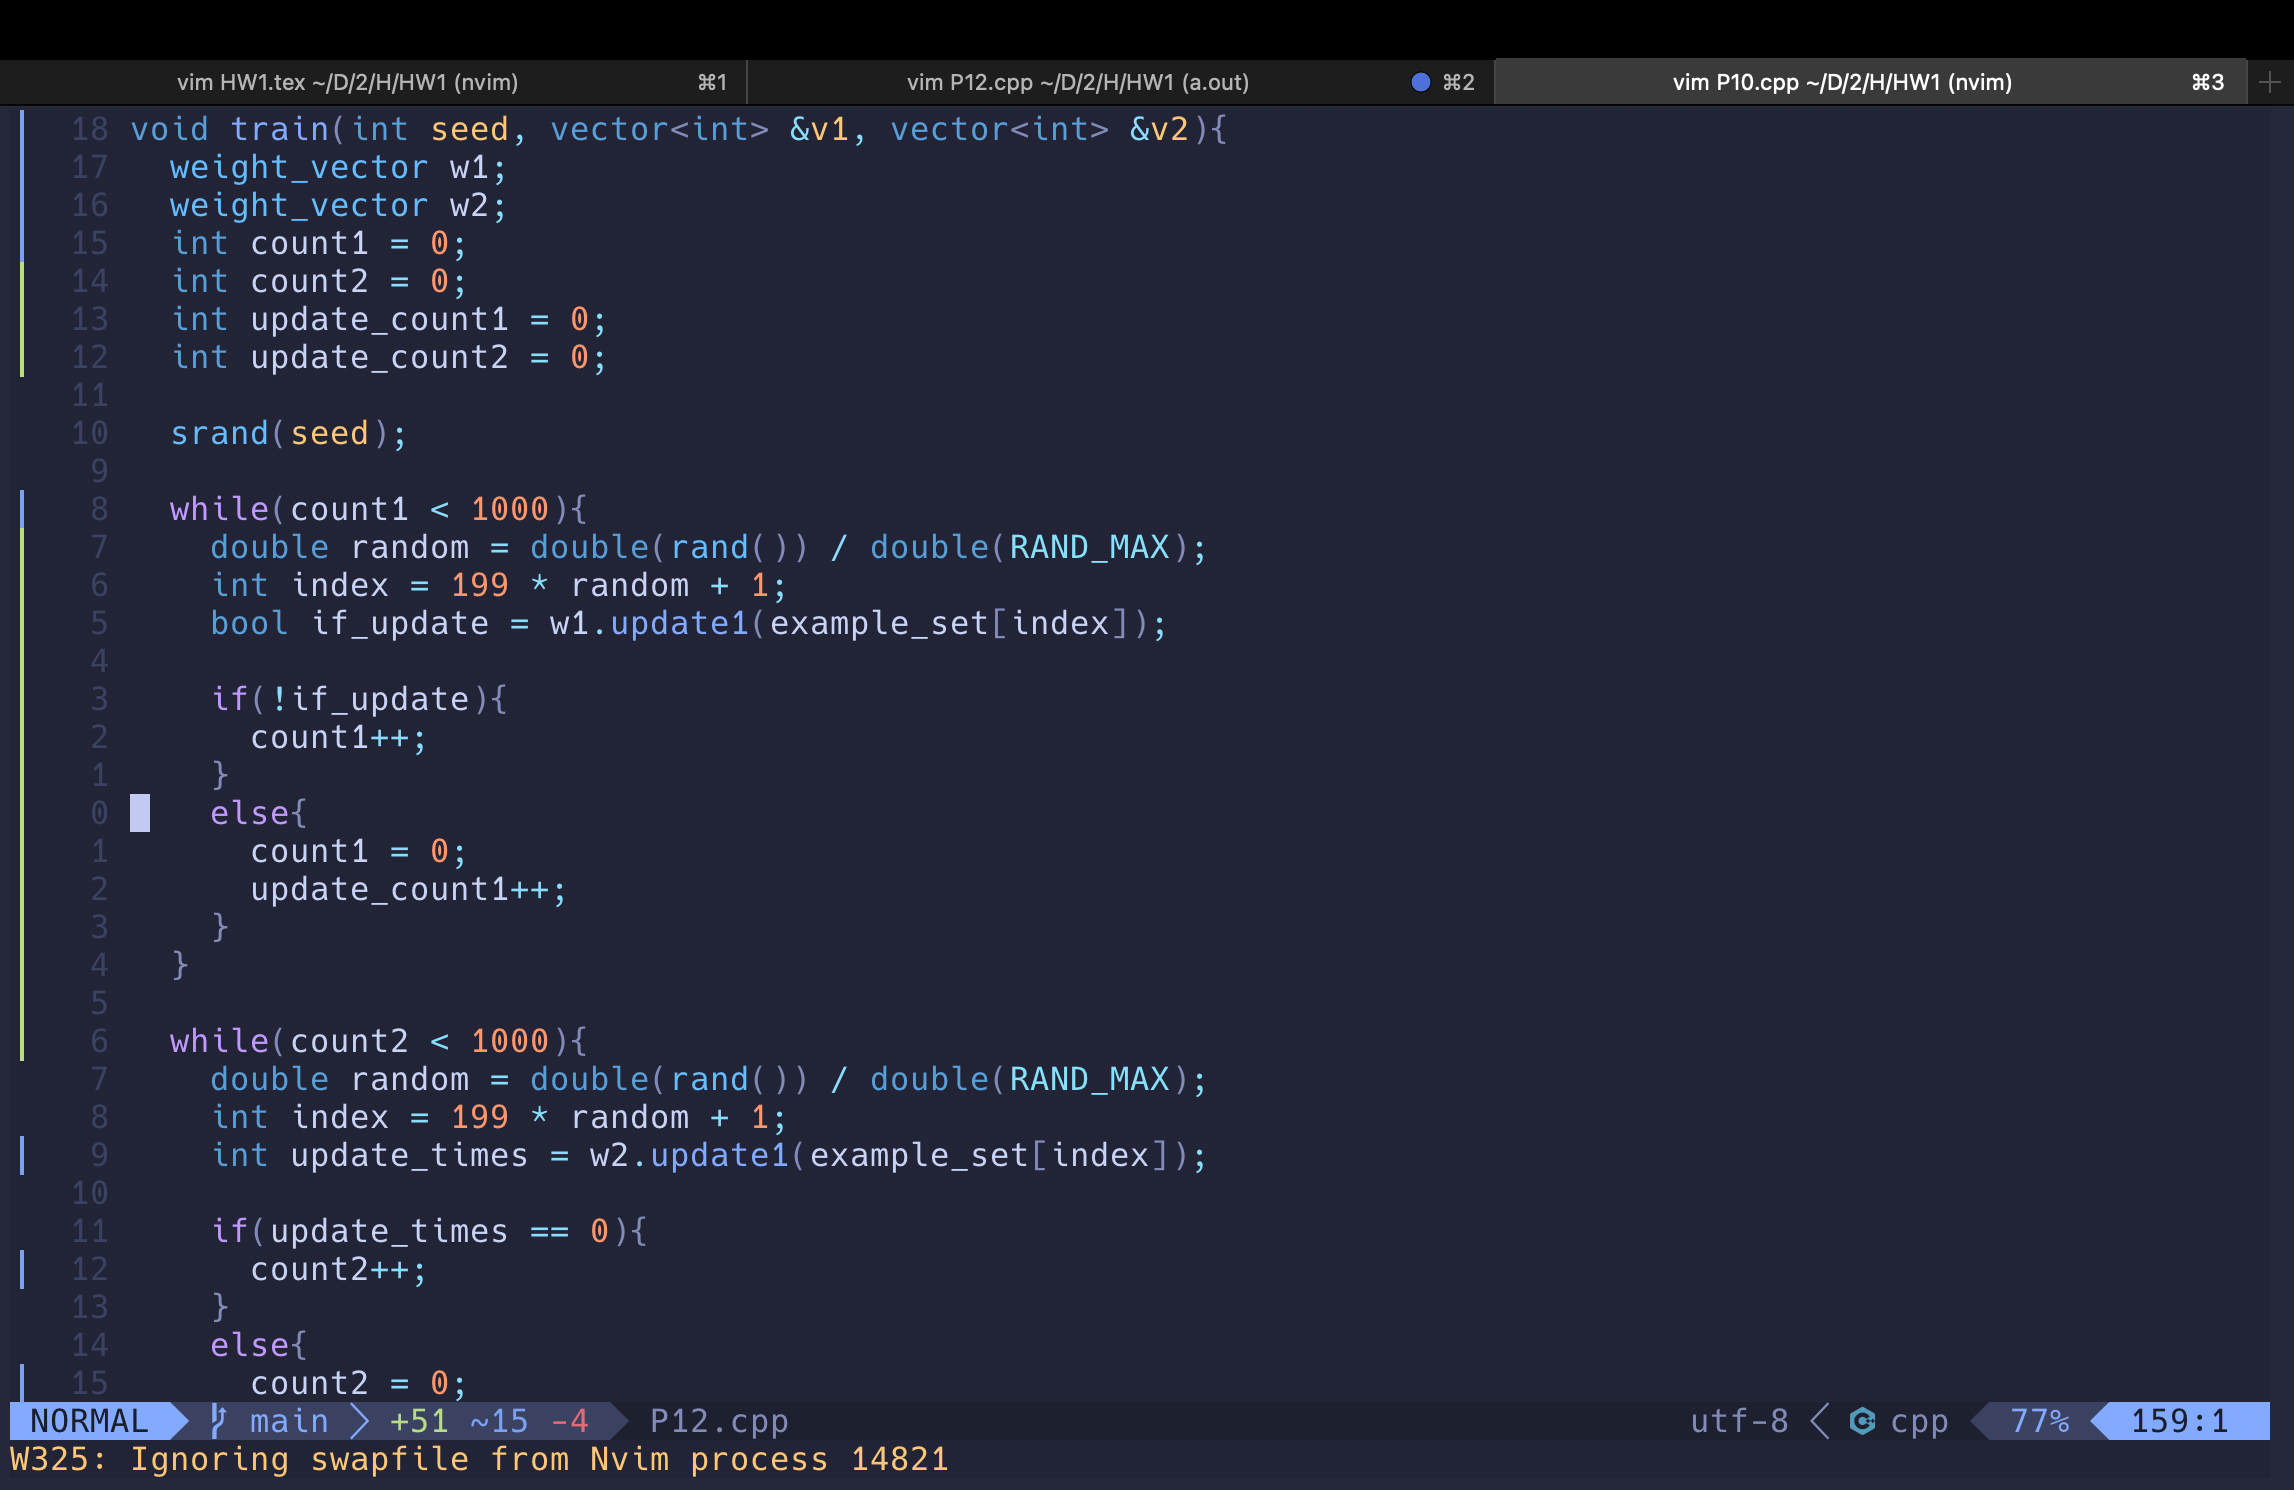
\includegraphics[width = \textwidth]{P12_code.png}\\
Code snapshot\\ 
Denote the result of one set of experiments as $(m_{10}, m_{12})$, where $m_{10}$ is the median of number of updates when running the algorithm in P10 and $m_{12}$ is that for P12. \\
The result is shown in the table below
\begin{center}
  \begin{tabular}{|c|c|c|c|c|}
    \hline 
    $(m_{10}, m_{12})$ & (101, 101) & (101, 102) & (102, 101) & (102, 102) \\ 
    \hline
    number of tests & 68 & 13 & 18 & 1\\
    \hline
  \end{tabular}
\end{center}
We see that the difference between the two PLA variants is quite insignificant for this dataset. Nevertheless, the number of tests where the variant in P10 outperforms that in P12(judging by median of number of updates) is higher than that of the opposite case. \\
A possible explanation to the similarity between the performance of the two PLA variants might be that since $\vb{w}^T\vb{x}$ is usually relatively small in this case, most of the time one update is enough to make the new $\vb{w}$ correctly classify the originally misclassified data point.
\newpage
\section*{13}
\subsection*{1}
First we consider how $\vb{w}_{t+1}$ classifies $\vb{x}_{n(t)}$ 
\begin{gather*}
  \vb{w}^T_{t+1}\vb{x}_{n(t)} = \vb{w}_t^T\vb{x}_{n(t)} + \frac{1}{10}y_{n(t)}\norm{\vb{x}_{n(t)}}^2\left\lfloor\frac{-10y_{n(t)}\vb{w}_t^T\vb{x}_{n(t)}}{\norm{\vb{x}_{n(t)}}^2} + 1\right\rfloor \\ 
   > \vb{w}_t^T\vb{x}_{n(t)} + \frac{1}{10}\norm{\vb{x}_{n(t)}}^2\frac{-10\vb{w}_t^T\vb{x}_{n(t)}}{\norm{\vb{x}_{n(t)}}^2} = 0
\end{gather*}
Hence sign($y_{n(t)}$) = sign($\vb{w}_{t+1}^T\vb{x}_{n(t)}$), and $\vb{x}_{n(t)}$ is correctly classified.  \\ 
\subsection*{2}
If the data is linearly separable, there exist a vector $\vb{w}_f$ such that 
\[
  \text{sign}(\vb{w}_f^T\vb{x}_n) = \text{sign}(y_n) \quad \forall (\vb{x}_n, y_n) \in \mathcal{D}
\]
% We first consider how $\vb{w}_f^T\vb{w}_t$ changes with $t$ 
% \begin{gather*}
%   \vb{w}_f^T\vb{w}_{t+1} = \vb{w}_t^T\vb{w}_t + \frac{1}{10}y_{n(t)}\vb{w}_f^T\vb{w}_t\left\lfloor\frac{-10y_{n(t)}\vb{w}_t^T\vb{x}_{n(t)}}{\norm{\vb{x}_{n(t)}}^2} + 1\right\rfloor \\ 
% \end{gather*}
\subsubsection*{2.1}
We first consider a different variant of PLA in which when $y_n\vb{w}_t^T\vb{x}_n \leq 0$ $\vb{w}_t$ is updated by
\[
  \vb{w}_{t+1}\leftarrow\vb{w}_t + \frac{1}{10}y_{n(t)}\vb{w}_{n(n)}
\]
(The condition that $y_n\vb{w}_t^T\vb{x}_n \leq 0$ is almost equivalent to the condition that the example is falsely classified, but it alleviates us from the trouble of dealing with convention for sign($0$)) \\
We then prove that this variant of PLA halts to a perfect hyperplane if the data is linearly separable. \\
Consider the inner product of $\vb{w}_t$ and $\vb{w}_f$ 
\begin{gather*}
  \vb{w}_f^T\vb{w}_{t+1} = \vb{w}_f^T(\vb{w}_t + \frac{1}{10} y_{n(t)}\vb{w}_t) \\ 
  \geq \vb{w}_f^T\vb{w}_t + \frac{1}{10}\min_n(y_n\vb{w}_f^T\vb{x}_n)
\end{gather*}
Next, we consider the change of the length of $\vb{w}_t$. 
\begin{gather*}
  \norm{\vb{w}_{t+1}}^2 = \norm{\vb{w}_t + \frac{1}{10}y_{n(t)}\vb{x}_{n(t)}}^2 \\ 
  = \norm{\vb{w}_t}^2 + \frac{1}{5}y_{n(t)}\vb{w}_t^T\vb{x}_{n(t)} + \frac{1}{100}\norm{\vb{x}_{n(t)}}^2
  \leq \norm{\vb{w}_t}^2 + \frac{1}{100}\max_n({\vb{x}_n}^2)
\end{gather*}
Now we consider the cosine value of the angle between $\vb{w}_T$ and $\vb{w}_f$ after $T$ updates, assuming that the process starts with $\vb{w}_0 = \vb{0}$
Let $\rho = \frac{\min_n(y_n\vb{w}_f^T\vb{x}_n)}{10\norm{\vb{w}_f}}$ and $R^2 = \max_n(\norm{\vb{x}_n}^2)$
\begin{gather*}
  \frac{\vb{w}_f^T\vb{w}_T }{\norm{\vb{w}_f}\norm{\vb{w}_T}} \\ 
  \geq \frac{T\rho}{\norm{\vb{w}_T}}
  \geq \frac{T\rho}{R\sqrt{t}} = \frac{\sqrt{T}\rho}{R}
\end{gather*}
Since the cosine value must be no greater than 1, we have
\begin{gather*}
  \frac{\sqrt{T}\rho}{R} \leq 1 \\ 
  \implies T\leq(\frac{R}{\rho})^2
\end{gather*}
We see that $T$ is upper-bounded, so this process halts with a perfect hyperplane. 
\subsubsection*{2.2}
Now we consider the same process, only that we keep using the same example for update(that is, $n(t+1) = n(t)$ until the crieteria for update is not met). \\ 
We now calculate the number of updates that is made with an example 
\begin{gather*}
  y_{n(t)}\vb{w}_t^T\vb{x}_{n(t)} + \frac{n}{10}\norm{\vb{x}_{n(t)}}^2 > 0 \\ 
  \implies n > -\frac{10y_{n(t)}\vb{w}_t^T\vb{w}_{n(t)}}{\norm{\vb{x}_{n(t)}}^2} \\ 
  \implies n = \left\lfloor-\frac{10y_{n(t)}\vb{w}_t^T\vb{w}_{n(t)}}{\norm{\vb{x}_{n(t)}}^2} + 1\right\rfloor
\end{gather*}
Hence after all the updates with one example $\vb{x}_{n(t)}$ is done, the new $\vb{w}$ is 
\[
  \vb{w} = \vb{w}_t + \frac{1}{10}y_{n(t)}\vb{x}_{n(t)}\left\lfloor-\frac{10y_{n(t)}\vb{w}_t^T\vb{w}_{n(t)}}{\norm{\vb{x}_{n(t)}}^2} + 1\right\rfloor
\]
This is identical to the way $\vb{w}$ is updated in the PLA invariant described in this problem.
\subsubsection*{2.3}
Now we see that the PLA variant described in this problem is equivalent to the one we proved to halt to a perfect hyperplane in the previous part, only that we choose the examples with which we update $\vb{w}$ in a special manner. From the proof presented in the previous part we see that how we choose the examples used for updates should not affect the fact that the process halts to a perfect hyperplane. Hence we've proven that this PLA process halts to a perfect hyperplane if the data is linearly separable.


\end{document}

